\subsection{Distributed comparator measurements}
We distribute native tool comparisons across Windows hosts because opening,
cleanup and saving are costly. Each result records its host, input identity,
configuration and timing boundary. Cross-tool ratios compare the same original
workbook with SheetShrink on the same host. Each host/tool combination is plotted
separately. Workload, tool behavior and session conditions still affect these
ratios. The frozen selection comprises the 49 workbooks with the largest absolute
compressed-file savings in each corpus's earlier SheetShrink screening. Results
apply to these selected cases.

NXPowerLite runs on a Lenovo 81YQ with a Ryzen 5 4500U (six cores and six logical
processors), 8 GiB installed RAM (7.37 GiB usable), a 512 GB Samsung MZALQ512HALU
NVMe SSD and Windows 11 Home build 26200. The power scheme is Energy Star.
Resource records include other open Excel and validation processes.

\paragraph{Comparator configuration}
NXPowerLite Desktop 11.0.1 x64 uses a custom Excel profile with only excess
cell-formatting cleanup enabled. All other cleanup options are disabled to
preserve visible content. An output audit checks whether images remain unchanged.

We compare media, drawings, charts and embedded objects byte-for-byte against the
originals. Of 147 workbooks, 129 became smaller and ten remained unchanged. Eight
Enron inputs failed with an internal NXPowerLite error, including after restarting
and retrying. Five outputs recompressed PNGs without changing decoded RGBA pixels
or dimensions. Another changed an embedded Word document. These six outputs are
retained separately and excluded from the formatting-focused timing figure. The
remaining 133 outputs passed the audit. Worksheet appearance still requires
separate visual validation.

XLStylesTool UWP 3.0.1.0 runs on the same host, with forced style normalization,
name unhiding and wholesale external-name removal disabled. We retain 122
hash-matched inputs with confirmed primary conversions and complete timing and
resource records. The other 25 inputs lack complete timing evidence and are
excluded. All 122 outputs preserve audited media and object parts byte-for-byte.
The joint figure uses the 110 inputs shared by both tools, comprising 21 Destatis,
41 Enron and 48 Data.gov workbooks, with the same repeated SheetShrink baselines.
Table~\ref{tab:top49-resources} reports NXPowerLite resources for all 133 audited
outputs.

Check Performance uses Excel 16.0.20527.20150 on the Lenovo host, with one
owned private-desktop Excel worker per input. Among the same 110 originals,
102 primary workflows completed (86 confirmed Optimize All actions and sixteen
no-optimization-needed outcomes), one was partial and seven failed, including
one timeout. Complete outcomes comprise 21 Destatis, 36 Enron and 45 Data.gov
inputs. The partial attempt saved an output before a progress-record replacement
failed; its successful diagnostic retry remains separate from primary statistics.
All original hashes matched before and after processing.

Check Performance wall time covers native-wrapper startup through exit,
including control saves, optimization, artifact creation and shutdown. Input
staging and independent hashing are excluded. Optimization and its associated
saves share one phase; their individual times are unavailable. Excel-only CPU
was retained through exit for all complete primaries, with working set and
private bytes sampled at a median mean interval of 251 ms. All 990 reused Lenovo
SheetShrink measurements list a concurrent Check Performance runner process;
these snapshots do not establish whether it was active. The median descriptive
workflow ratios are 20.19, 22.75 and 4.84 for Destatis, Enron and Data.gov.
Background-load uncertainty and different endpoints qualify these ratios.

The Inquire lane uses an HP EliteBook 645 G11 with an AMD Ryzen 5 PRO 7535U
(six physical cores, twelve logical processors), 32 GiB installed RAM,
a 512 GB SOLIDIGM NVMe SSD and Windows 11 Enterprise build 26200.9711.
Excel and Inquire file versions are 16.0.17932.21056 and 16.0.16626.20076.
Of the same 110 originals, 90 have full primary Inquire successes, six partial
outcomes and fourteen failures. Diagnostic retries remain separate. Full
successes comprise 19 Destatis, 28 Enron and 43 Data.gov workbooks.

Inquire records single historical Excel workflow observations, including opening,
cleanup with internal saving, explicit saving and shutdown; detailed boundaries
remain in the per-case receipts. Partial and failed attempts receive no
completed-runtime ratio. Historical hardware and version attribution partly
uses execution-session provenance and later inventory rather than per-trial
capture. Among the 90 complete pairs, 41 Inquire work directories were on local
NVMe, 48 on a USB-connected Samsung 870 QVO SSD, and one has incomplete storage
attribution. All paired SheetShrink trials used local NVMe. The source receipts retain these storage conditions. The median descriptive workflow
ratios are 19.36, 15.18 and 12.04 for Destatis, Enron and Data.gov, respectively.
Different endpoints and storage conditions constrain their interpretation.

The HP SheetShrink lane freezes revision \texttt{75e85035}, twelve Rayon and
twelve writer workers, and one active workbook. One warm-up precedes seven
measured trials per input, extended to eleven when the relative interquartile
range exceeds 10\%. All 110 inputs completed: 110 warm-ups and 806 measured
trials, with identical uncompressed output contents across repetitions for each
input. Trials used fresh native Windows processes, warm filesystem caches,
seeded shuffled ordering and a 1,800 s timeout. Hashing and verification are
outside process-start-to-exit timing. The host retained its institutional power
scheme and background workload. No comparator Excel process ran concurrently
with these timed SheetShrink trials.

\paragraph{Timing and resources}
Each NXPowerLite and XLStylesTool observation has one primary timing measurement per input. Its operational cost
limits replication, and its timing variability therefore remains unestimated.
Diagnostic retries remain separate attempts. Elapsed time covers automated GUI
orchestration through output confirmation and initial package verification.
CPU measurements accumulate attributed process-tree user and kernel time.
Working-set and private-byte peaks use a nominal 250 ms sampling interval. The existing warm
application is reused, with one conversion worker and a 512 MiB RAM and commit
reserve.

The Lenovo SheetShrink experiment uses an optimized release build from revision
\texttt{765c480}, one active workbook, one Rayon worker and one writer, with the
default cleanup policy. One complete warm-up round precedes nine measured rounds
over the same 147 source identities. Each round independently shuffles workbook
order with a recorded seed. Each file starts a fresh CLI process, and measured
wall time ends at process exit. Output hashing is outside this timing boundary.
Filesystem caches are left unflushed after warm-up. Direct-child CPU and OS peak-working-set counters
are retained, with private usage sampled at a nominal 10 ms polling interval. These memory observations
have different sampling semantics from the GUI lane and are reported separately.
All 1,470 invocations completed successfully. Each input produced the same
package hash across warm-up and measured repetitions, and all 147 final outputs
preserved the original bytes of the audited media and object parts.
Across inputs, the median relative within-input interquartile range,
$(Q_3-Q_1)/\widetilde{t}$, was 0.84\% over the nine measured repetitions.

Figure~\ref{fig:paired-cleanup-workflows} retains raw times and workbook-level
same-host ratios. Each denominator is the same-host SheetShrink median (nine Lenovo trials or
seven to eleven HP trials),
and each numerator is the primary comparator observation. Across-workbook quartiles
describe heterogeneity in this deliberately selected stress panel. They are
distinct from uncertainty over repeated trials~\cite{scientificbenchmarking}.
The ratio includes the stated interface and confirmation costs, and the tools
have different cleanup policies. It therefore measures the observed cleanup
workflows. Opening-time improvements and cleanup-plus-opening costs require
their own readiness endpoints, as in the separate historical opening experiment.

\begin{table*}[t]
\caption{Median resource observations across paired workbooks on the laptop.
CPU is process time in seconds.
WS is working set in MiB, using OS peak counters for Sheet Shrink and sampled peaks for NXPowerLite.}
\label{tab:top49-resources}
\centering
\setlength{\tabcolsep}{3pt}
\begin{tabular}{lrrrrr}
\hline
Corpus & Pairs & CPU Sheet Shrink & CPU NXPowerLite & WS Sheet Shrink & WS NXPowerLite \\
\hline
Destatis & 44 & 1.24 & 5.45 & 54 & 248 \\
Enron & 41 & 0.70 & 4.19 & 51 & 306 \\
Data.gov & 48 & 6.73 & 10.49 & 415 & 146 \\
\hline
\end{tabular}
\end{table*}


\begin{figure}[t]
\centering
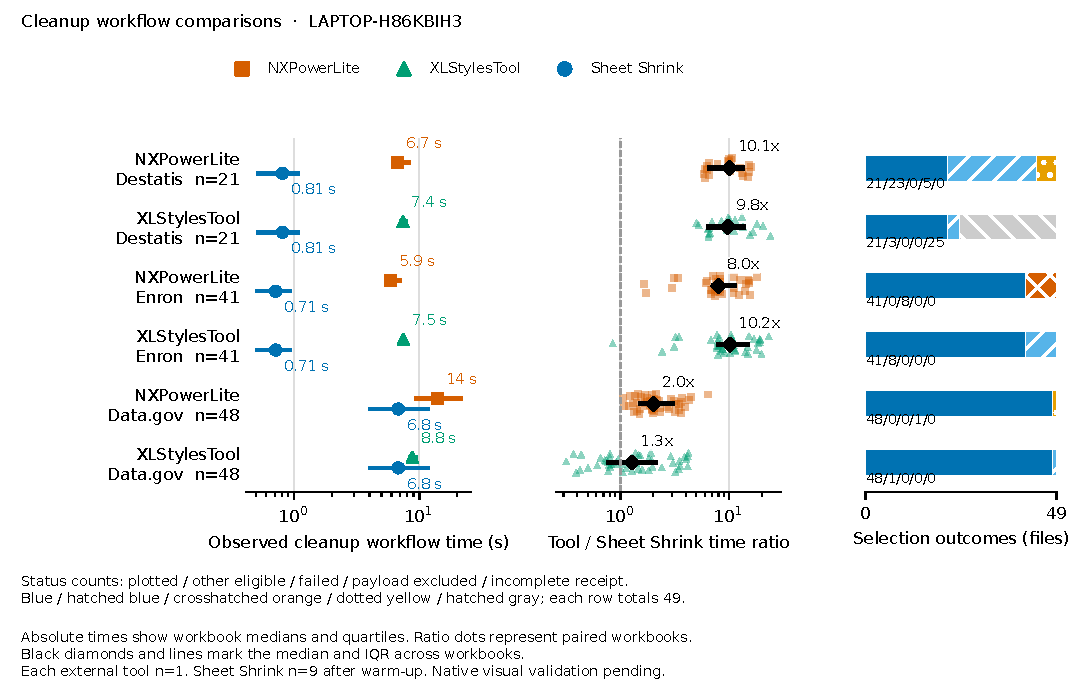
\includegraphics[width=\columnwidth]{figures/paired-cleanup-workflows.pdf}
\caption{Cleanup times and tool/SheetShrink ratios by corpus; parentheses give
pair counts. Time summaries and black ratio marks show medians and interquartile
ranges. NXPL: NXPowerLite; XLST: XLStylesTool; CP: Check Performance; INQ: Inquire.}
\label{fig:paired-cleanup-workflows}
\end{figure}
